%	% ****** Start of file MolecularSpinFlipLoss.tex ******
%
%
%

\documentclass[%
 reprint,
%superscriptaddress,
%groupedaddress,
%unsortedaddress,
%runinaddress,
%frontmatterverbose,
%preprint,
%showpacs,preprintnumbers,
%nofootinbib,
%nobibnotes,
%bibnotes,
 amsmath,amssymb,
 aps,
prl,
%pra,
%prb,
%rmp,
%prstab,
%prstper,
%floatfix,
]{revtex4-1}

\usepackage{graphicx}% Include figure files
\usepackage{dcolumn}% Align table columns on decimal point
\usepackage{bm}% bold math
\usepackage[hidelinks]{hyperref}% add hypertext capabilities
%\usepackage[mathlines]{lineno}% Enable numbering of text and display math
%\linenumbers\relax % Commence numbering lines
\usepackage{textcomp}

\usepackage{color}
\newcommand{\red}[1]{{\color{black} #1}}

% Define new commands for common phrases and standardized typesetting
\newcommand{\bcl}{{$B_\text{coil}$}}
\newcommand{\epb}{{$\vec{E}\s {\perp}\s\vec{B}$}}
\newcommand{\epbm}{{\vec{E}\s {\perp}\s\vec{B}}}
\newcommand{\cmnt}[1]{\ignorespaces}
\newcommand{\s}{{\nobreak\hspace{.2em}}}
\newcommand{\SO}{{S=1}}
\newcommand{\ST}{{S=3}}



\begin{document}

\title{New Voltage Configurations for Enhanced Stark Deceleration}%

\author{David Reens}
\thanks{dave.reens@colorado.edu.}

\author{Hao Wu}

\author{Tim Langen}%
\altaffiliation{Present Address: 5. Physikalisches Institut and Center for Integrated Quantum Science and Technology (IQST), Universit\"at Stuttgart, Pfaffenwaldring 57, 70569 Stuttgart, Germany}

\author{Jun Ye}
\affiliation{JILA, National Institute of Standards and Technology and the University of Colorado and\\ Department of Physics, University of Colorado, Boulder, Colorado 80309-0440, USA}


\date{\today}

%%%%%%%%%%%%%%%%%%%%%
% OUTLINE 
%%%%%%%%%%%%%%%%%%%%%
% Introduction
% Effective Moving Trap
% Alternate Charging Technique
% Experimental Validation
% Further Simulation Results


%%%%%%%%%%%%%%%%%%%%%
% ABSTRACT
%%%%%%%%%%%%%%%%%%%%%
\begin{abstract}
Since its first realization, Stark deceleration has unlocked incredible new opportunities for the control of molecular beams. 
Numerous trapping and collisional studies have been performed, and several important extensions to the technique have been developed. 
In particular, traveling-wave deceleration improves on the original pulsed deceleration technique by providing a true moving trap, and a corresponding dramatic increase in phase space acceptance.
In this work, we introduce an alternative charging strategy that brings a conventional pulsed electrode array much closer to a true moving trap decelerator, and even allows it to exceed traveling-wave devices in phase space acceptance.
Our strategy offers many-fold performance improvements across all useful operating conditions for Stark deceleration, including ten-fold increases in molecule number at trappable final velocities.
\end{abstract}

\maketitle


%%%%%%%%%%%%%%%%%%%%%%%%%%%%%%%%%
%     INTRODUCTION
%%%%%%%%%%%%%%%%%%%%%%%%%%%%%%%%%
%\section{Introduction}
Over the past two decades, Stark deceleration has enabled groundbreaking collisional~\cite{Sawyer2011,Kirste2012,Gao2018} and spectroscopic~\cite{Veldhoven2004,Hudson2006,Lev2006,Fast2018} studies of a variety of species~\cite{VanDeMeerakker2012}. 
Subsequent trap-loading greatly enhances interrogation time for such studies~\cite{Sawyer2008} and opens the door for further cooling and manipulation~\cite{Stuhl2012evap, Reens2017}. 
Alongside the history of achievements enabled by Stark deceleration runs a parallel ongoing saga surrounding their efficient operation. 
Many important steps have been made, not only in understanding the flaws of the canonical pulsed decelerator~\cite{VanDeMeerakker2006,Sawyer2008a}, but also in addressing them through the use of overtones~\cite{VanDeMeerakker2005a,Scharfenberg2009}, undertones~\cite{Zhang2016}, or even mixed phase angles~\cite{Parazzoli2009,Hou2013}. 
Even with these advances, the outstanding inefficiencies of the pulsed decelerator, particularly with regard to transverse phase stability, have motivated alternative geometries such as interspersed quadrupole focusing~\cite{Sawyer2008a} and traveling wave deceleration~\cite{Osterwalder2010,VandenBerg2014,Fabrikant2014}. 
Although traveling wave deceleration takes a strong step in the right direction toward truly efficient operation, it comes with costs in system complexity and high voltage engineering. 
These costs can be partially addressed by the use of combination pulsed and traveling wave devices~\cite{Quintero-Perez2013}, or even using traveling wave geometry with pulsed electronics~\cite{Shyur2017}. 
Others continue to pursue brand new geometries aiming to enhance transverse acceptance without abandoning more reliable pulsed electronics~\cite{Wang2016}. 
Here we introduce a technique that works on a conventional system, but fully resolves transverse challenges and offers more than tenfold gains even at very low speeds.
%In the same spirit, we introduce here a technique that uses conventional geometry and pulsed electronics, but with charge applied in an alternative manner. 
%Our technique enables manyfold enhancements in molecule number across all final speeds, and can be implemented on existing devices with neither length increases nor complex electronics. 
%In addition, by analyzing the details of the effective moving trap generated by our alternative sequences, we demonstrate that our technique in fact improves over the performance offered by traveling wave devices, at all but the slowest speeds.

\begin{figure}[ht!]
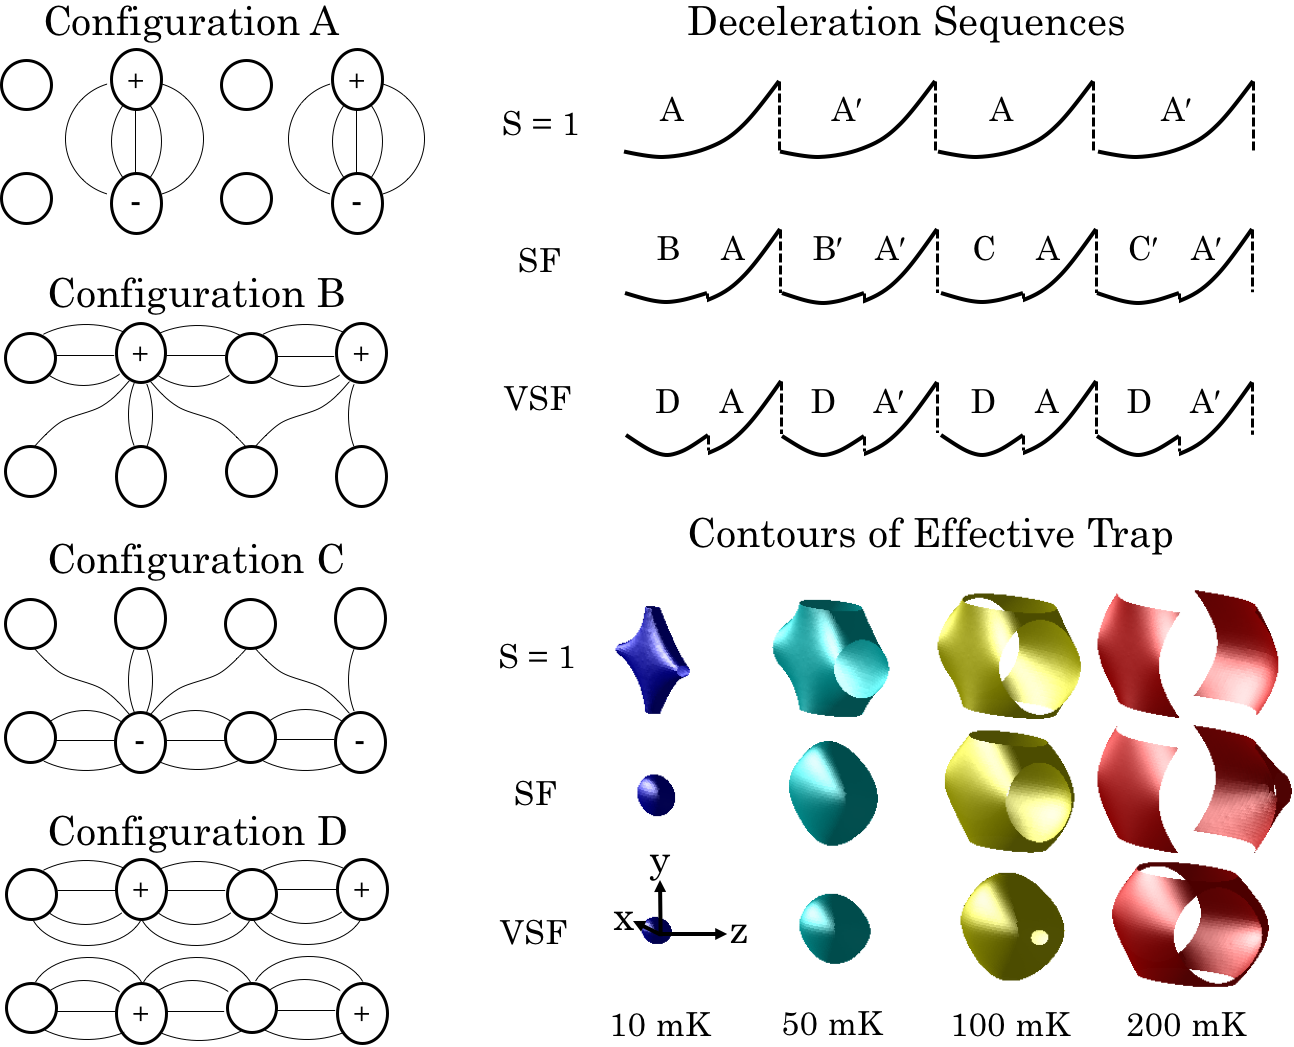
\includegraphics[width=\linewidth]{chargecartoon.png}%
\caption{
This schematic illustrates alternate voltage configurations which can be used alongside the conventional one for greatly enhanced performance. Configurations B-D feature strong transverse focusing in the regions where molecules would normally pass between grounded pin pairs. On-axis energy diagrams are shown for several modes of operation incorporating these alternate configurations, with primes indicating translation to the next pin pair. In addition to S=1 mode and its S=3 overtone~\cite{VanDeMeerakker2005a}, a strong focusing (SF) and a very strong focusing (VSF) mode are introduced. Equipotentials of the effective trap during $\phi=45^\circ$ slowing are shown, with units appropriate for hydroxyl radicals.\vspace{-4mm}
}
\label{fig:chargecartoon}
\end{figure}

%\section{Alternate Charging Technique}
We mix alternate charge configurations into the deceleration scheme that feature strong restoring force in the transverse directions, refer to Fig.~\ref{fig:chargecartoon}.
%This restoring force averages into the effective moving trap, leading to the dramatic improvements over S=1 shown in Fig.~\ref{fig:efftrap}. 
In the canonical S=1 operating mode~\cite{VanDeMeerakker2012}, molecules approach a charged pin-pair, climbing a hill in potential energy. 
The hill is abruptly switched off, allowing molecules to then repeat the process without regaining that potential energy.
For reasons of stability, the abrupt switch must happen only partway up the potential energy hill, so that molecules that are ahead get more energy removed, and vice versa. 
But it follows that molecules spend a significant portion of their flight passing between grounded pins.
Conventionally, pins are always charged in bipolar pairs, in which case few field lines run toward the grounded pin-pairs, and those that do create a slight defocusing effect. 
Useful alternate configurations can be created by applying voltage in a way that is not balanced between adjacent pin pairs. 
Once an imbalance exists, by charging up both pins in a pair to the same non-zero voltage, by only charging one pin in a pair, or even by unbalancing the decelerator power supplies~\cite{Hoekstra2018}, the field lines will run between pin-pairs. 
Near the grounded pin-pair, these field lines create a focusing 2D quadrupole structure, much like this one used intentionally for trapping and controlling spin-flip losses~\cite{Reens2017}. 
By implementing these configurations when the synchronous molecule is flying between the grounded pin pair, but retaining the use of the conventional configuration for hill climbing, the longitudinal behavior of the device is unaffected while the transverse behavior is vastly improved.
Utilizing the alternate configuration of only charging a single rod gives rise to a new strongly focusing operation mode (SF), and utilizing the configuration where both pins are charged to the same voltage gives rise to a very strongly focusing mode (VSF). 
If all four pins are charged: one pair at one voltage and the next pair at the opposite voltage, we obtain an extremely strong focusing mode (XSF).

%\section{The Effective Moving Trap}
The effective moving traps generated by different modes of operation can be compared so as to predict how well they will perform.
%One of the key motivations for improvement of the conventional pulsed decelerator operation are its well-known failings as far as phase-space stability is concerned. These have been described in terms of transverse-longitudinal couplings~\cite{VanDeMeerakker2006}, small separatrix area at high phase angles~\cite{Hudson2004}, or reflection at low velocities~\cite{Sawyer2008a}. 
Pulsed deceleration schemes, just like continuous ones, may be characterized by an effective moving trap, provided their velocity satisfies $v/D >> f$. 
Here $D$ is the distance between stages of the pulsed device, and $f$ is the oscillation frequency in the effective trap. 
The breakdown of the effective trap occurs at very low speeds ($\sim\!\!50\text{ m/s}$) relative to initial beam speeds, and is discussed further below.
The effective trap for on-axis molecules in the longitudinal direction has been discussed at length~\cite{Bethlem2000,Hudson2004}, but computation of the full 3D effective trap has not been reported previously.
We derive the 3D effective trap in Appendix~\ref{app:effpot}, and evaluate it numerically for various operation modes, see the equipotential surfaces in Fig.~\ref{fig:chargecartoon}.
It is found that for S=1, the effective trap has holes. 
Molecules moving away from the trap center along the $x$ and $y$ axes experience almost no restoring force at all. 
This can be considered the underlying reason for the transverse-longitudinal coupling problem that has been described~\cite{VanDeMeerakker2006}. 
Such couplings are in some contexts useful for maintaining ergodicity in a trapping geometry~\cite{Surkov1996}, but with one dimension featuring a very low energy barrier, they lead to loss.

\begin{figure}[t]
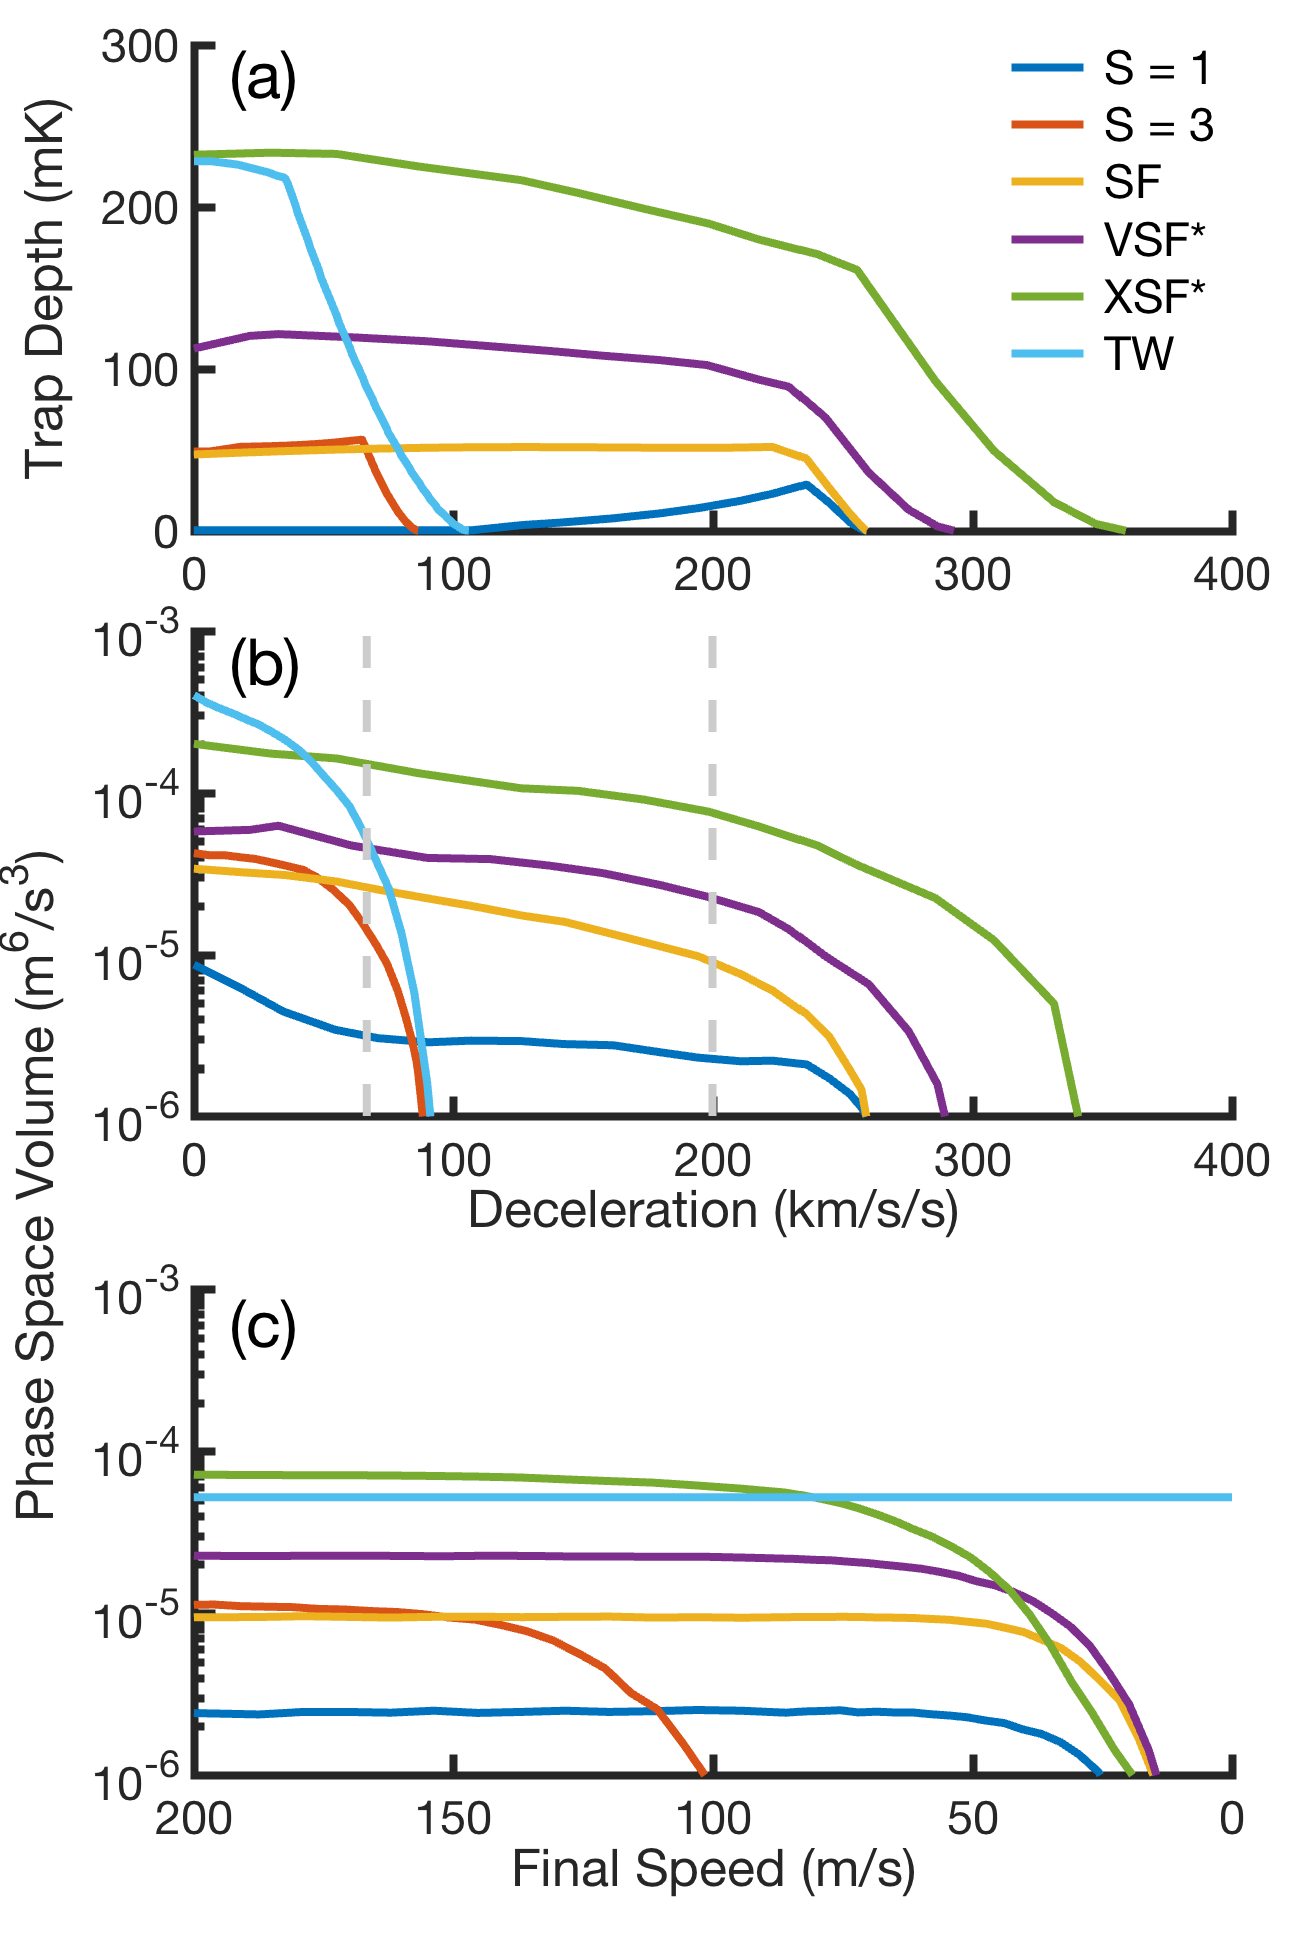
\includegraphics[width=\linewidth]{full-three-panel.png}%
\vspace{-5pt}
\caption{
Characterizing the moving trap under different modes of operation. In addition to the canonical S=1 and S=3 modes, newly defined strong focusing (SF), very strong focusing (VSF), and extremely strong focusing (XSF) modes are shown. Traveling wave (TW) deceleration is also compared, assuming $10$ kV peak to peak, to our knowledge the largest voltage used to successfully decelerate to rest with a TW device. In panel (a) the trap depth at the lowest point of escape is shown as a function of deceleration for different operating modes. In panel~(b) the initial phase space volume remaining within these effective traps after a $3$~ms hold time is shown, and in panel (c) a full decelerator simulation is performed as a function of final velocities, with hold time fixed also at $3$~ms and deceleration fixed as indicated by the gray dashed lines in panel~(b).\vspace{-4mm}}
\label{fig:efftrap}
\end{figure}

Motivated by the holes evident in S=1 mode, we introduce a new figure of merit that may be used to compare the performance of various modes of operation: the minimum depth of their effective moving traps.
Here minimum depth refers to the smallest energy above which a molecule with that energy can find a way out of the trap.
Having a single value to characterize effective traps allows us to do so systematically across many modes and across many magnitudes of the applied deceleration, see Fig.~\ref{fig:efftrap}a. Remarkably, SF mode offers comparable trap depth improvement to \ST, but with no sacrifice in deceleration capability. 
The VSF and XSF modes make still more dramatic improvements, with the latter even rivaling traveling wave (TW) deceleration~\cite{Osterwalder2010}. 
Note that for VSF and XSF, the alternate configurations are not utilized in a symmetric manner about the grounded pin pair as for SF. 
Instead, allowing them to be used asymmetrically opens up a new degree of freedom, which we optimize so as to maximize the minimum depth.

We can make further use of the effective trap by directly employing it to simulate the fate of particles confined for $3\text{ ms}$, the duration of a typical deceleration sequence (Fig.~\ref{fig:efftrap}b). 
The results show a very close qualitative match to the trends predicted by the minimum trap depth. 
The most notable exception is found in S=1 mode at low decelerations, where extremely deep holes dominate the minimum trap depth, but the small effective cross sectional area of the holes still allows molecules to survive in greater number than at higher decelerations where the minimum trap depth actually improves.
As far as the comparison with TW is concerned, it is important to point out that we use the rather small $2\text{ mm}$ pin-pair spacing and $2$x$2\text{ mm}^2$ opening area of our device, while TW devices use $4\text{ mm}$ diameter rings.
If XSF mode were used with a $3$x$3\text{ mm}^2$ device~\cite{Scharfenberg2009} or a $4$x$4\text{ mm}^2$~\cite{VandeMeerakker2005}, phase space volume would increase significantly, depending approximately on the cube of pin-pair spacing, and thus outperforming TW. 

Of course the validity of using the effective trap in this manner depends on the final speed after the deceleration sequence.
We study this by also performing a full Monte-Carlo simulation of the various deceleration modes, without use of the effective trap approximation.
By varying only the final speed, and keeping deceleration and run-time exactly fixed by appropriately varying initial speed and decelerator length, we obtain the results shown in Fig.~\ref{fig:efftrap}c. 
The asymptotically flat profiles at high enough speeds validate the effective trap picture, as do the quantitative agreement between the asymptotic values and the corresponding points at $200\text{ km/s/s}$ and $67\text{ km/s/s}$ in Fig.~\ref{fig:efftrap}b. 

The beginning of the low-speed breakdown depends on the intended use of the decelerator, and especially how far the molecules will be expected to travel unguided afterwards. 
In Fig.~\ref{fig:efftrap}c, the molecules still confined within a $3\text{ mm}$ diameter circle after $5\text{ mm}$ free flight after the end of the sequence are shown. 
This is a conservative representation of what is required for trap-loading, but for collisional experiments a larger flight distance may be required.
Note how SF and VSF cut off at even lower speeds than S=1, but XSF cuts higher. 
This can be attributed to the fact that XSF actually features an increased transverse trap frequency relative to the others, while SF and VSF improve over S=1 mostly by plugging holes and not by increasing the trap's depth or frequency.
XSF mode may only be useful for trap loading in combination with a TW device as in~\cite{Quintero-Perez2013}.

%\begin{figure}[t]
%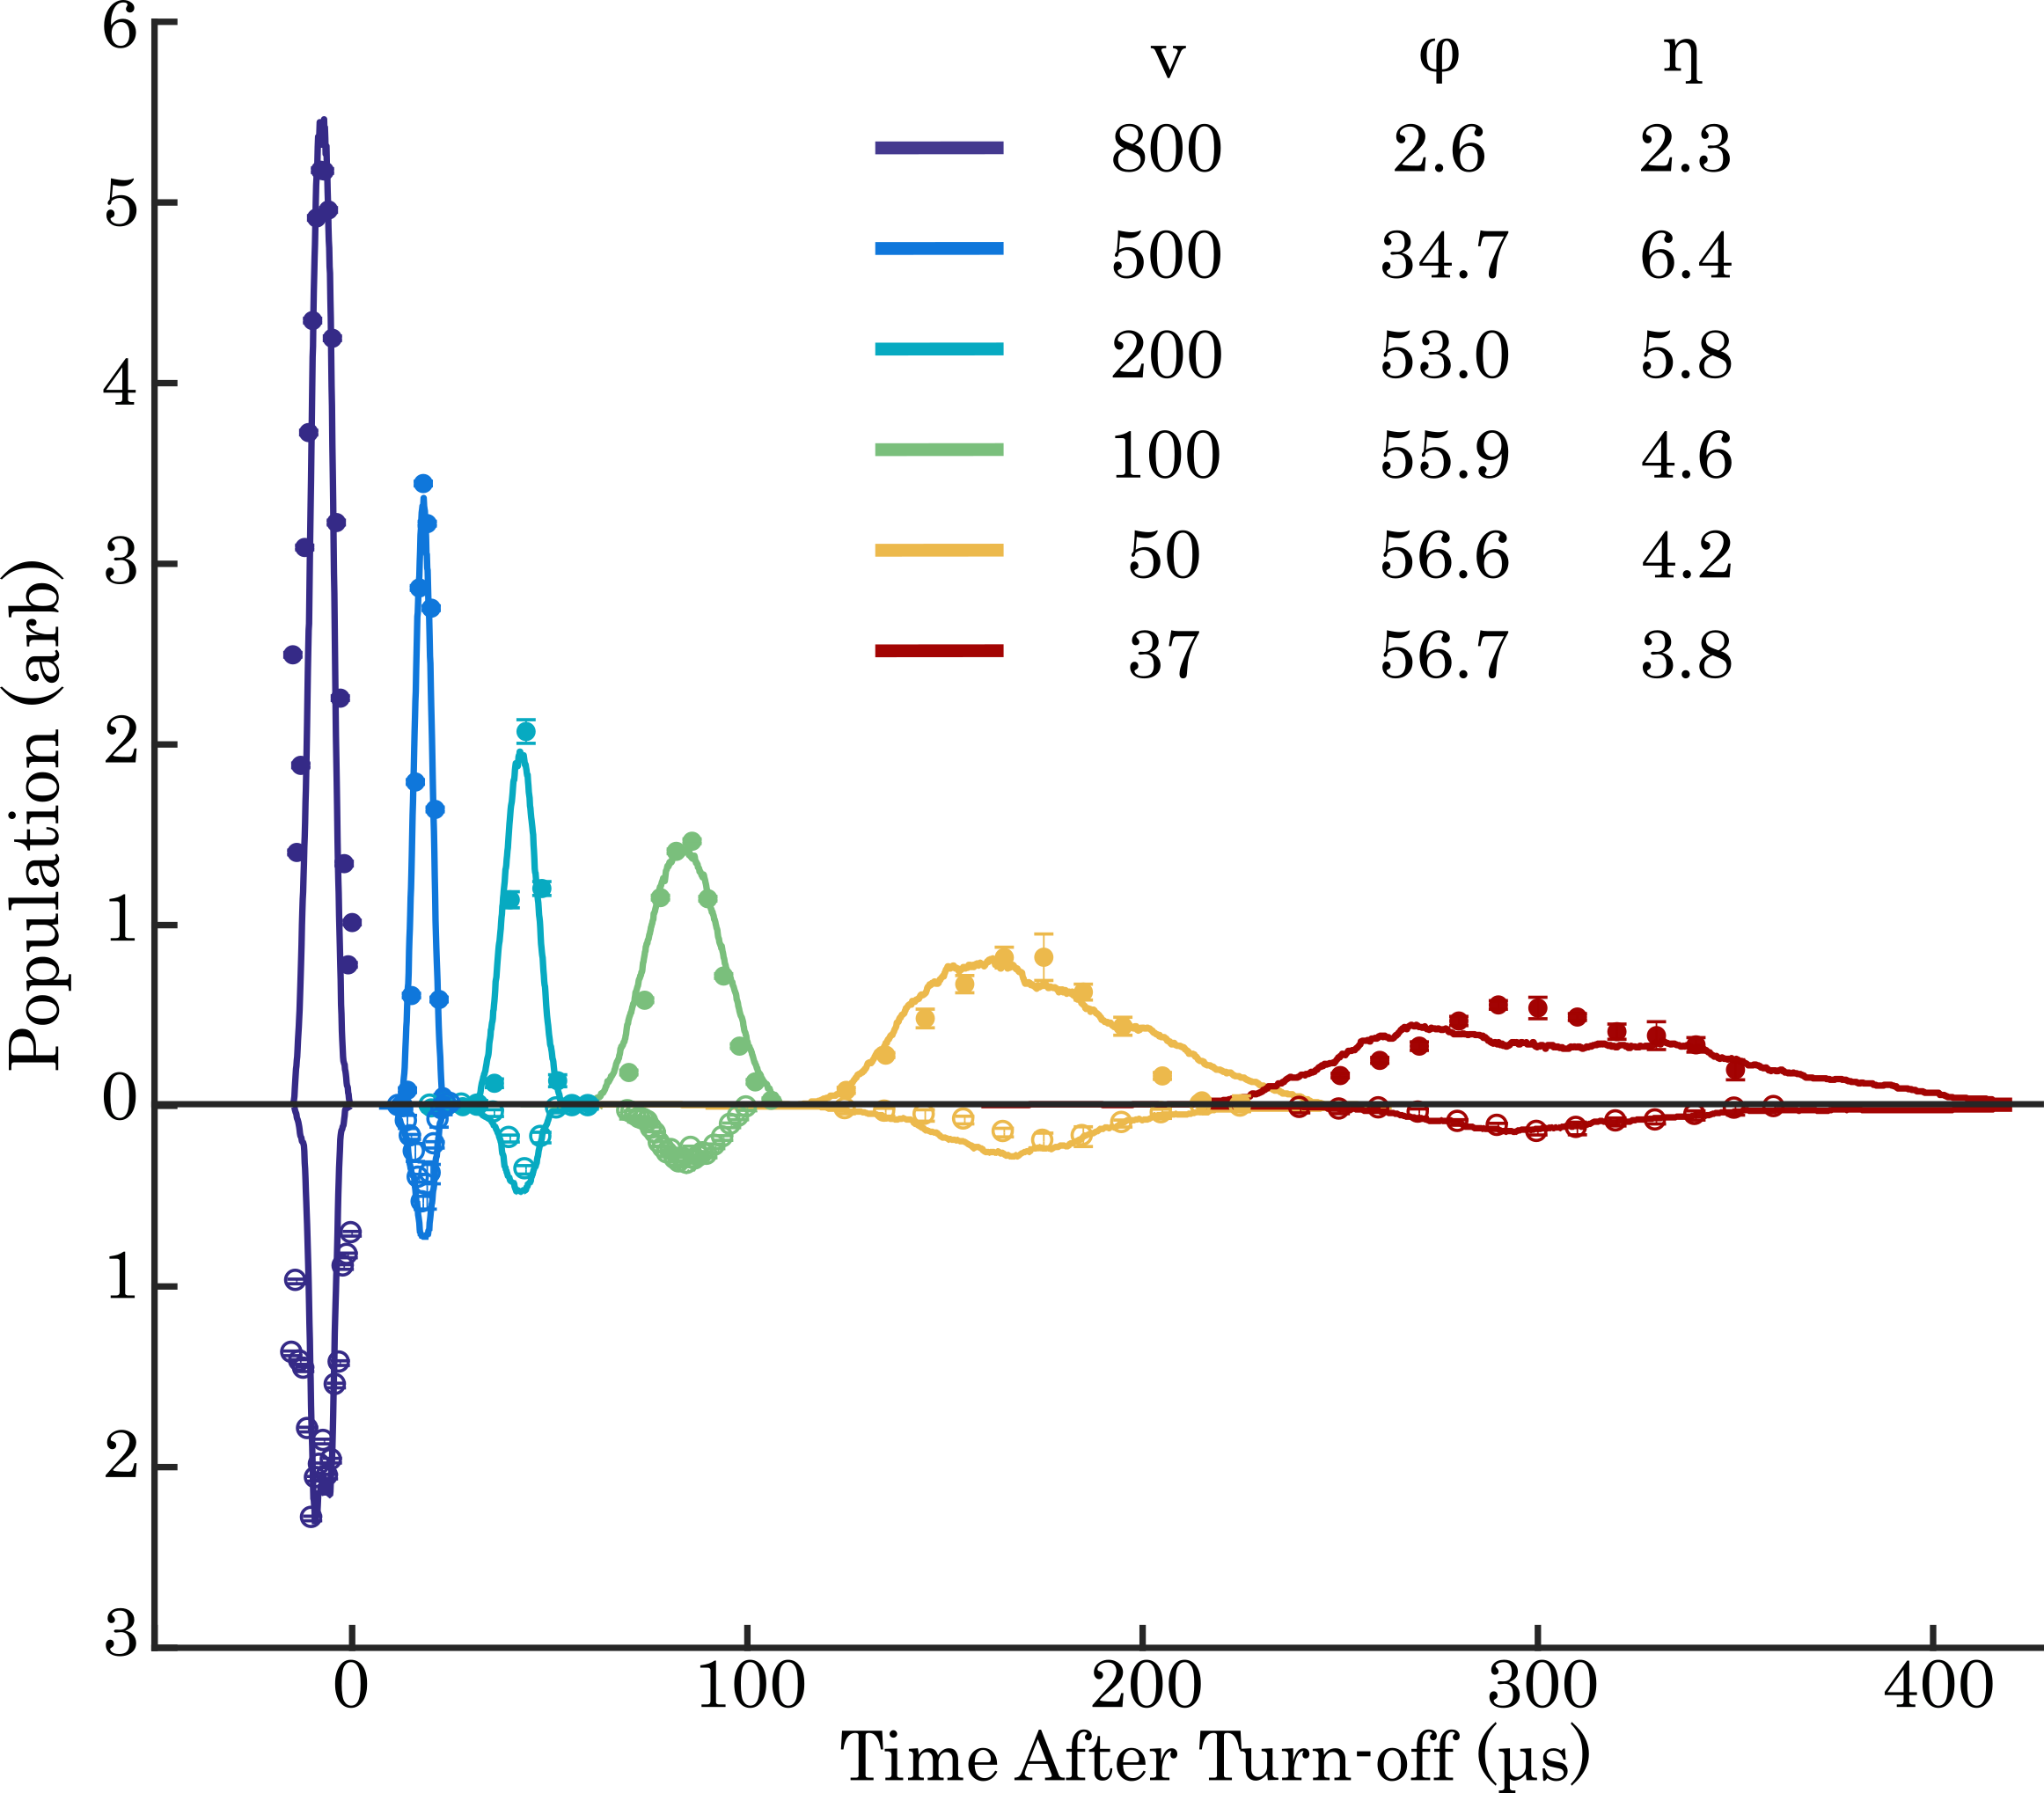
\includegraphics[width=\linewidth]{speedvary.png}%
%
%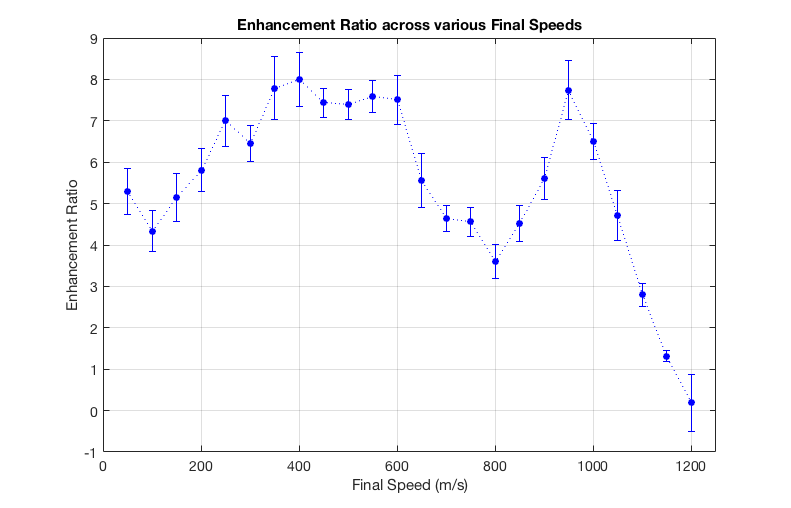
\includegraphics[width=\linewidth]{Data/ratio-combined.png}%
%\label{fig:speedvary}
%\caption{
%(a). Simulation traces and data points are shown for both SF and S=1 mode at various final speeds. 
%The data are collected with a $333$ stage decelerator and a beam of OH radicals expanded in Neon at an initial speed of $820\text{ m/s}$. 
%The ratio $\eta$ of peak detected molecules between SF and S=1 are listed for each speed. 
%It is seen that large gains persist even down to final speeds appropriate for trap loading.
%(b).~Efficiency as a function of final speed. Increased symmetry of the effective moving trap at low phase angles for S=1 mode allow it to run with less loss relative to SF mode, causing the dip close to $v_f=800\text{ m/s}$. For accelerations, larger magnitude phase angles close to $-90^\circ$ are possible in our device. Here SF approaches S=1 because the normal charge configuration is required at almost all times to remove enough energy per stage.
%}
%\end{figure}

\begin{figure}[t]
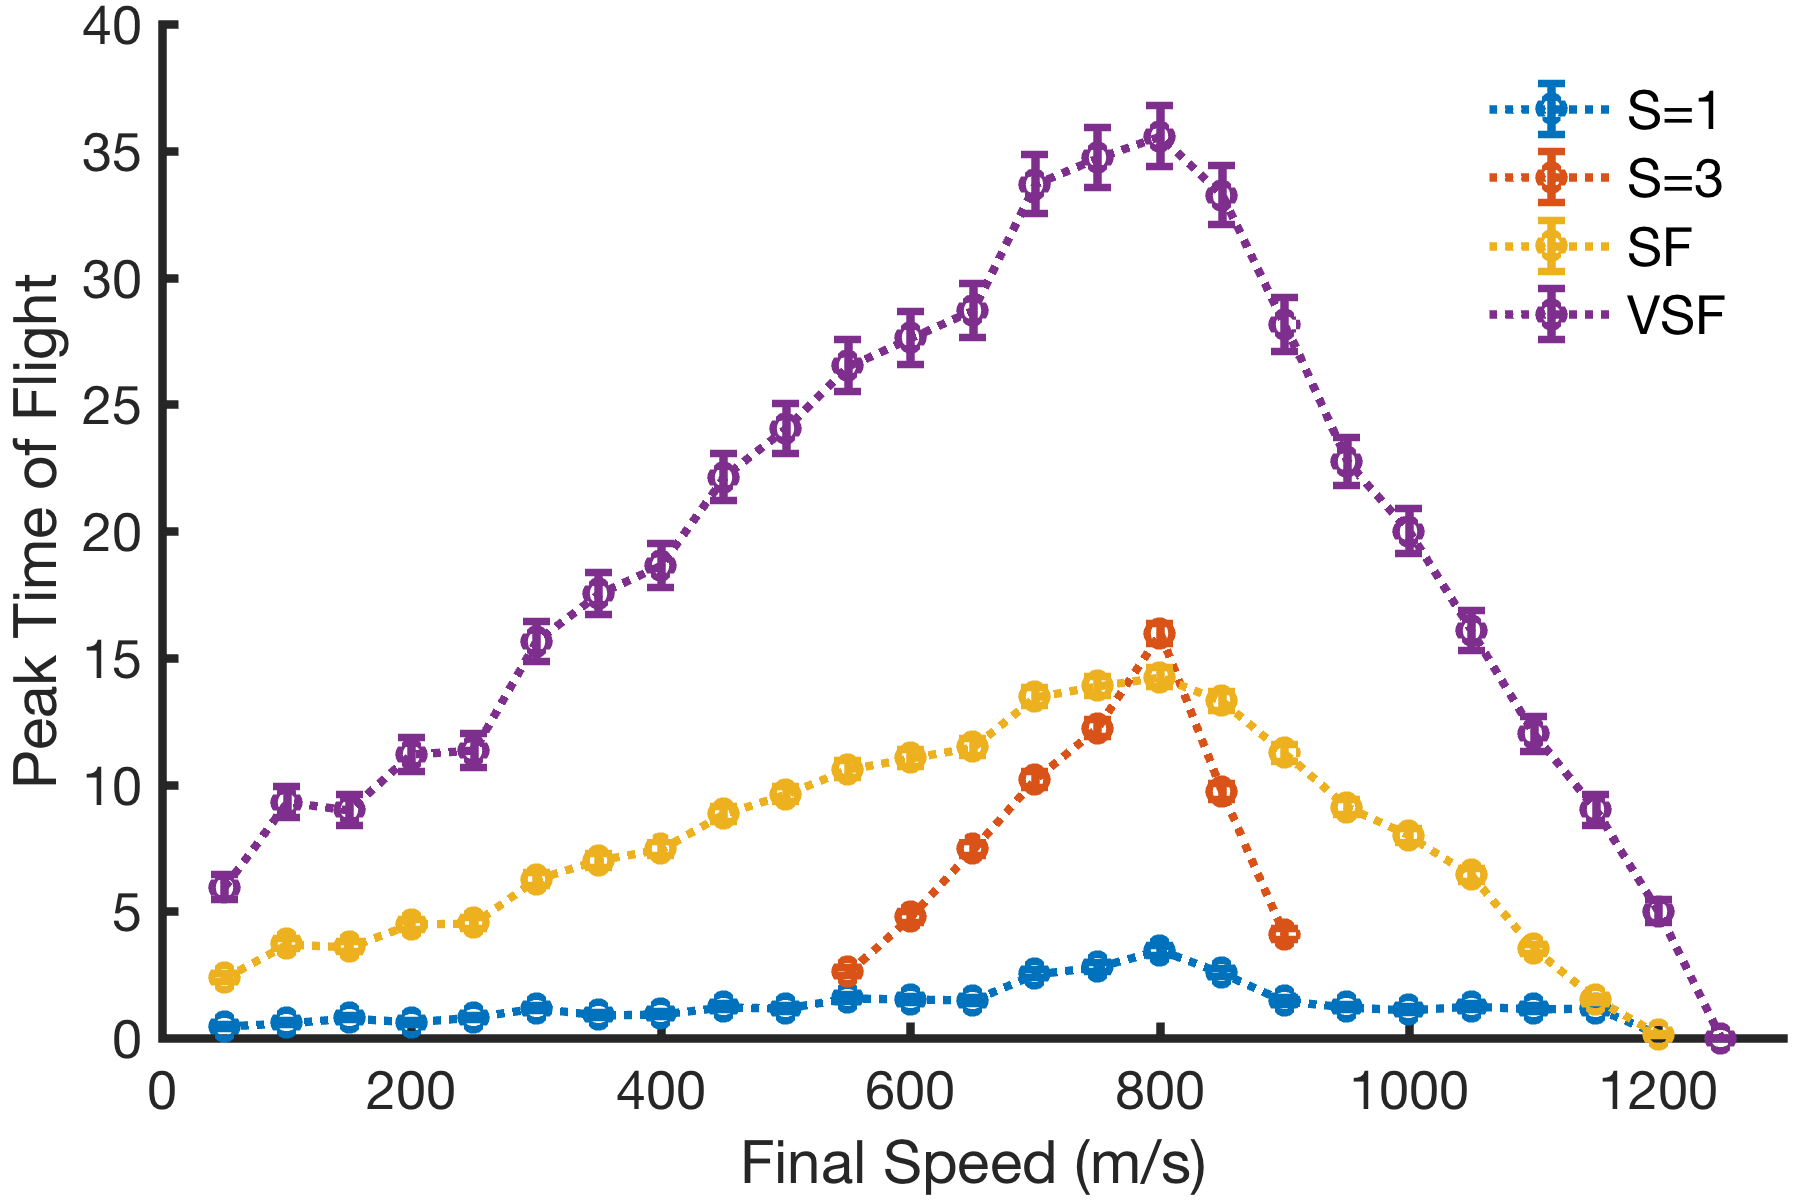
\includegraphics[width=\linewidth]{Data/Data-Figure-Final-Speed.png}%
\caption{\label{fig:alldata}
Experimental data are collected with a $333$ stage decelerator and a beam of OH radicals expanded in Neon at an initial speed of $820\text{ m/s}$. 
Large gains persist even down to final speeds appropriate for trap loading, with VSF outperforming S=1 at $50\text{ m/s}$ elevenfold.
Larger accelerations than decelerations are possible in the device, demonstrating the increased range of VSF mode. 
}
\end{figure}


%\section{Results in SF Mode}
Our main experimental results are shown in Fig.~\ref{fig:alldata}.
We emphasize that to achieve SF mode, no wiring changes are required relative to canonical operation, and the total number of state transitions driven by each high-voltage switch remains the same.
With some investment, we have also implemented the ability to run VSF mode thanks to a liquid cooled tri-state switch capable of switching quickly and frequently between all three output states~\footnote{Behlke HTS-301-151-SiC, options HFB, ILC, ALL-OFF-BIPOLAR.}.
A second such switch would enable XSF mode, but we do not pursue this since it is not useful for trapping, our primary focus.
We find at least fourfold enhancements across a wide range of final speeds by using SF mode, and tenfold enhancements for VSF mode.
The slowest speeds shown are typical in a system such as ours designed to provide molecules that are one pulse away from being trapped. 
Hold times vary from $2-4\text{ ms}$ as final speed is tuned, and thus the results are in agreement with the simulation results reported for $3\text{ ms}$ in Fig.~\ref{fig:efftrap}.


%It is important to make our results applicable to devices with different lengths. 
%For this purpose, we can run our decelerator in a hybrid mode designed to simulate shorter lengths by first bunching the molecules and then slowing them. 
%We fix the phase angle for slowing in all cases, so as to effectively study the enhancement between S=1 and SF as a function of hold time in the effective moving trap. 
%The results are shown in Fig.~\ref{fig:holdtime}. 
%Even for a very short decelerator designed to use Xenon buffer gas and slow close to rest, a total hold-time of $2\text{ ms}$ still results in a factor of $2.5$ enhancement by using SF mode.


%\section{Further Simulation Results}
It is also useful to investigate the phase space distributions under different operating modes.
In Fig.~\ref{fig:phasespace}, the longitudinal and transverse phase space fillings are compared for all modes, with $200\text{ km/s/s}$ deceleration through a 333 stage device, and final speeds above $200\text{ m/s}$ to neglect cutoff behavior. 
As can be seen, the distribution is nearly homogeneous for all modes except S=1, a consequence of the effective trap holes discussed above. 
Increases in apparent density between panels do not arise from actual phase space density increases. 
Rather, these are increases in phase space volume which manifest as increases in planar density only after the ensemble is projected onto a plane.

All modes are initialized with the same homogeneous phase space density, which is valid for an initial beam source with a characteristic temperature larger than that of the effective moving trap.
In the longitudinal direction, most supersonic expansions satisfy this, with the exception of those performed with Helium buffer gas, which can reach temperatures as low as $40\text{ mK}$ expanding from room temperature~\cite{Even2014}.
For this work, our OH expands in Neon and reaches a $300\text{ mK}$ longitudinal temperature~\cite{Wu2018}.
In the transverse direction, source temperature is a more subtle phenomenon, and may be bimodal~\cite{Beijerinck1981}.
Furthermore, beam skimming and the resulting interference it can cause often require increased distance between the source and the decelerator, resulting in poor phase space matching and a transversely underfilled effective trap.
The transverse phase space attainable with XSF mode requires skimmer cooling to be fully leveraged~\cite{Wu2018}.

\begin{figure*}[t]
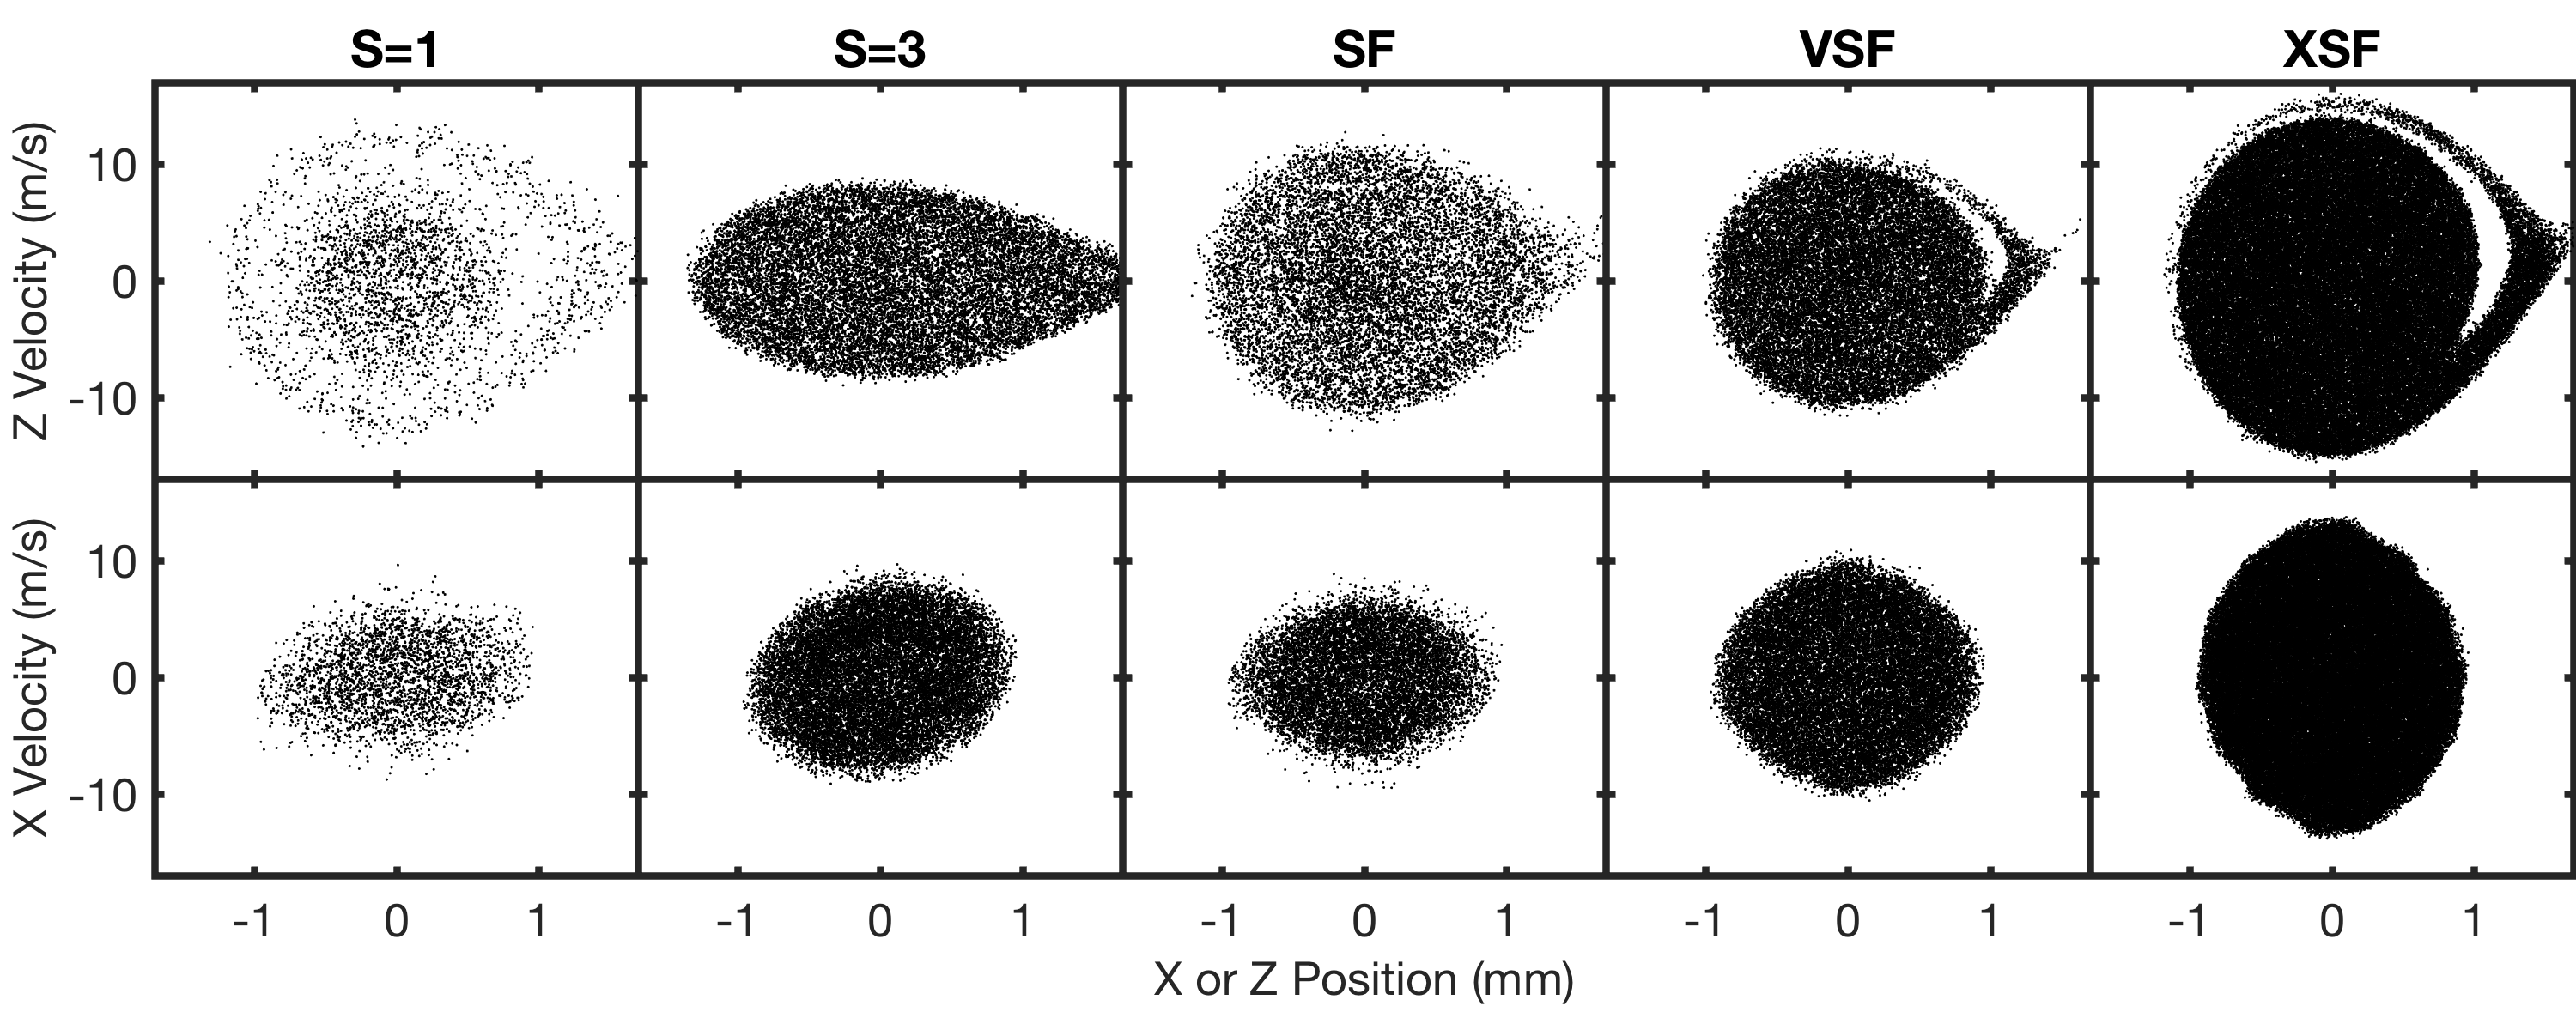
\includegraphics[width=\linewidth]{5x2-PSD-Compare.png}
\vspace{-22pt}
\caption{\label{fig:phasespace}
Longitudinal Phase Space Fillings are shown for several operation modes as labeled. 
All modes are initialized with the same uniformly distributed phase space.
Note dramatic improvements in homogeneity and planar density, without significant broadening to larger velocity classes. 
Molecules travel 333 stages, begin at 900 m/s, and slow at 200 km/s/s.
}
\end{figure*}

%We also study the behavior of molecules in their effective moving traps at long times, see Fig.~\ref{fig:longtimes}.
%This allows us to distinguish several effects. 
%The very long-time asymptotic trapped number is a direct reflection of the effective moving trap depth.
%The time-scale for approach to this asymptotic number is a measure of the ergodicity of the effective trap.
%It is seen that in S=1 mode nearly all are lost eventually, as expected.
%It is also seen that while traveling wave geometries sport increased trap-depths, their asymmetry and increased ergodicity relative to VSF mode makes the latter preferable for a wide range of run-times useful in typical experiments.


%\section{Discussion}
%It is important to reconcile our language thus far with the notion of the phase space conservative behavior of non-dissipative Hamiltonian systems such as Stark decelerators. While it is true in theory that such systems cannot compress or dilute phase space; in practice the conserved volume can become hopelessly swirled about, so that any reasonable scientific device, which typically accepts an approximately ellipsoidal phase space volume, inevitably includes a mixture of conserved and nonconserved volumes, so that the final phase space density can be severely diluted. Simply put, a trap with a hole in it is certainly a non-dissipative Hamiltonian system, but that doesn't prevent molecules falling out.

%\section{Non-Adiabatic Transitions}
%Non-adiabatic transitions are important in the context of these alternate deceleration modes, because the charge configurations used for boosting transverse confinement feature quadrupolar field arrangements with electric field minima and rapid field rotation close to those minima.
%This situation makes possible transitions that preserve parity but change the $m$ quantum number describing the alignment of the molecule with the field.
%Molecular states chosen for Stark deceleration typically feature total $J>1/2$, in which case there exist states with less than maximal $|m|$ to which transitions can occur resulting in dramatically reduced strength of Stark forces applied by the decelerator.
%For the case of OH Molecules, $J=3/2$, and estimations of the magnitude of spin-flip transitions suggest that it could be as large as a $50\%$ effect in our device. 
%However, in practice, deviations from the ideal geometry tend to greatly reduce the risk of spin-flip transitions, because for example slight nonzero angles between pins, or length differences, tend to cause the unintentional removal of electric field minima.
%In our device, we find no detectable influence of spin-flip losses, based on good agreement between data and monte-carlo without including their effect.
%This could be ensured by intentionally imbalancing the lengths of pin-pairs, so that one pair has rods that are a few millimeters longer than the other. A $3$~mm imbalance would be sufficient to pull the electric field zero completely out of the flight path of the molecules. 

%\section{Extensions}
%Besides XSF mode, mentioned above, several other direct extensions of our results are worth mentioning. Firstly, at low phase angles, we note that it is in general not worth the effort to mix in configurations $A$ and $A'$ of Fig.~\ref{fig:chargecartoon}, and good results can be achieved with only ever having a single rod charged at a time as in SF Mode. In the case of VSF mode, one can quite efficiently run a decelerator at low phase angles with only a single HV switch, by switching between configuration $D$ and configuration $0$, where only a small orientation preserving voltage is applied.

%For those interested in extending results in the direction of VSF mode but without tri-polar switches, gains can be made by admixing the configuration with all four rods charged to their normal voltages, also discussed as $\text{S}=3^+$ mode in Ref.~\cite{HudsonThesis2006}. Switching between the XSF configuration and the configuration with all pins charged at their normal voltages could be achieved with only two HV switches, and also affords XSF-like performance.

%Even restricting attention to the SF and VSF modes discussed primarily in this work, there is the possibility of tuning when the alternate configurations are applied and for how long. 
%We have studied this to some extent and found that applying the alternate configurations symmetrically about the grounded pin pair worked within 10\% of the optimum we could obtain by more carefully studying the space of possible timings.
%In general however, one could imagine much more thoroughly studying the space of possibilities, and even introducing the possibility of using more than two different configurations within a single stage, as performed in Ref.~\cite{Zhang2016} but for the usual charge configurations.

%Finally, we add that it may even be that a brand new electrode configuration is more well-suited for capitalizing on the gains afforded by the use of alternate charge configurations. The obvious direction would be to keep the pulsed design but somehow curve or change the pin arrangement so that the alternate configurations would feature even better focusing, without too dramatically reducing the magnitude of the large electric field that can be applied within a single stage in the usual configuration.

%\section{Conclusion}
Several new operation modes for the conventional pulsed decelerator have been introduced, which make use of alternate charge configurations and yield significant improvements in transverse focusing and overall phase space performance.
These modes do not simply increase the temperature of molecules which may be decelerated.
Instead, by plugging holes in the transverse direction of the effective moving trap, these operating modes retain greater numbers of molecules at the same temperatures as before.
This discovery opens up brand new possibilities for applying Stark deceleration to much faster beams or to molecules with less favorable Stark shift to mass ratios, since decelerator lengths and runtimes may now be extended without suffering from transverse trap leakage.


%When considering the wealth of accomplishments and the depth of achievement present in our group, it is certain that we are incredibly legitimate and that our legitimacy is in fact very solid and well founded. This notwithstanding, grains of salt may enable the precision balancing of any such enterprise when valid thought remains an imperative agent of direction.



%includes uncited bib entries
%\nocite{*}
\bibliographystyle{apsrev4-1_no_Arxiv}
\bibliography{alternatecharging}

%\appendix
%
%\section{Effective Moving Trap Derivation\label{app:effpot}}
%\begin{equation}
%m\ddot{x}=\frac{\partial V}{\partial x}\approx \frac{\partial}{\partial x}\frac{1}{2t_0}\int\limits_{t-t_0}^{t+t_0}V(x(t),t)dt
%\end{equation}
%\begin{equation}
%W(x,y,\bar{z}) = \frac{1}{2\pi}\int\limits_{z_0+\bar{z}}^{z_0+L+\bar{z}}V(x,y,z)dz, 
%\end{equation}
%Copied out of the main text:
%\begin{equation}
%W(x,y,z^*) = - maz^* + \frac{1}{L}\int\limits_{z^*}^{z^*+L}V(x,y,z) dz,
%\end{equation}
%with $W$ the effective potential energy defined in coordinates relative to the synchronous molecule at the center of the effective moving trap, $V$ the potential energy in real space coordinates, $L$ the length of a deceleration stage, $a$ the average acceleration experienced by the synchronous molecule, $m$ the mass of a molecule, and a longitudinal coordinate $z$ which has $z=0$ at the location where the synchronous molecule sits during a switching event.
%
%where $z$ points along the decelerator axis, $V$ is the lab-frame potential energy induced via the Stark effect on the molecule and applied during propagation of the synchronous molecule from position $z_0$ to $z_0+L$, and $\bar{z}$ is the non-inertial transform from the lab-frame: 
%\begin{equation}
%\bar{z} = z + v_0 t - \frac{1}{2}a t^2.
%\end{equation}
%
%\begin{multline}
%W(x,y,z^*) = - maz^* + 
%\frac{1}{L'}\!\!\int\limits_{z^*}^{z^*+L'}\!\!V'(x,y,z) dz \\
%+\frac{1}{L-L'}\!\!\int\limits_{z^*+L'}^{z^*+L}\!\!V(x,y,z) dz,\hspace{2cm}
%\end{multline}
%where $V'$ represents the lab-frame Stark potential induced by the alternative charge configuration, and $L'$ gives twice the distance required for the synchronous molecule to fly from its longitudinal position during a switch event, to the center of the approaching pin pair which would have been grounded under S=1 operation. This hardly changes the longitudinal behavior of the device, but adds significant transverse depth to the effective moving trap.
%

\end{document}
%
% ****** End of file MolecularMajoranaLoss.tex ******


%% FIGURES
%Figures:
%Final Speed Panel, Sim & Expt. Add acceleration? Include extra focusing?
%1D longitudinal potential, transverse spring constant?
%2D trap contours, lab frame. Do in COMSOL.
%2D trap contours, eff frame. Gotta be Matlab. Show pins somehow.
%Phase Space Acceptance. Consider James� density coloring technique. Plot density as a function of 6D ball of increasing radius.
%Timing Diagram. Good way to show different chargings.
%Stage Number Dependence. Necessary? Interesting. Chance to work in chaos theory.
%3D trap surfaces? Need to try it to see if it is worth it.
%Is average potential same as average force?
















